\chapter{INTRODUÇÃO}
\label{c.introducao}

A presença das redes de computadores no cotidiano vem aumentando de modo muito
veloz há anos e apresentou um crescimento em especial com o advento das redes
sem fio e da produção massiva e a queda do custo de dispositivos portáteis
capazes de se conectarem à internet. De maneira proporcional, aumentaram-se
também os riscos relacionados à segurança de redes e à privacidade de
informações de diversas espécies que trafegam por entre elas e seus usuários.
Numa proposição inicial, este trabalho define como \textit{Malware} todo tipo de
programa que seja capaz de alterar o comportamento de um software num
dispositivo conectado a uma rede qualquer, feito com o desejo de vender
informações de usuários, causar desordem, roubar credenciais, enviar spams,
alimentar motores de otimização de busca (SEO) com informações falsas sobre
visitas a páginas da Web ou ainda de chantagear usuários, como foi o caso do
\textit{malware} japonês denominado \textit{Kenzero}, que publicava históricos de navegação
juntamente com a identificação de seus usuários, a menos que os mesmos
pagassem 1500 ienes para que seus dados fossem retirados do acesso ao público.
SAWLE et al. (\citeyear{sawle14}).

De acordo com IDIKA (\citeyear{idika07}), pode-se classificar os tipos de
métodos de detecção de maneira mais rudimentar em duas categorias: detecção
baseada em anomalia e detecção baseada em assinatura. A detecção por anomalia
é uma técnica que consiste em treinar um algoritmo de deteção para que ele
“saiba” o que constitui o comportamento normal de um programa, para que ele
possa decidir sobre a periculosidade dos programas a serem inspecionados. Essa
mesma abordagem também dá origem a uma técnica muito similar conhecida como
detecção baseada em especificações, onde levantam-se especificações e
conjuntos de regras para que a partir daí defina-se o comportamento de um
programa normal. A técnica de detecção por assinaturas, por sua vez, envolve a
caracterização do que já seria sabidamente malicioso para encontrar traços
semelhantes e encontrar os programas anômalos. Todas as técnicas citadas acima
podem ser aplicadas com um de três modos diferentes, sendo eles análise
estática, análise dinâmica e análise híbrida, onde a análise estática num
contexto de detecção por assinaturas, verificaria aspectos estruturais de
programas inspecionados, como sequências de \textit{bytes}, e a análise dinâmica
buscaria informações de maneira concorrente ao tempo de execução do programa.
Em suma, a análise estática procura investigar o programa antes que ele seja
executado, e a análise dinâmica atua ou na execução do programa, ou depois que
ele já foi executado. As técnicas híbridas são simplesmente combinações dessas
duas anteriores, juntando informações estáticas e dinâmicas para que se
conclua um parecer sobre a maliciosidade dos códigos analisados.

Dessa maneira, é possível exemplificar as técnicas de deteção com a figura:

\begin{figure}[H]
\caption{\small Classificação das técnicas de detecção de \textit{Malware}}
\centering
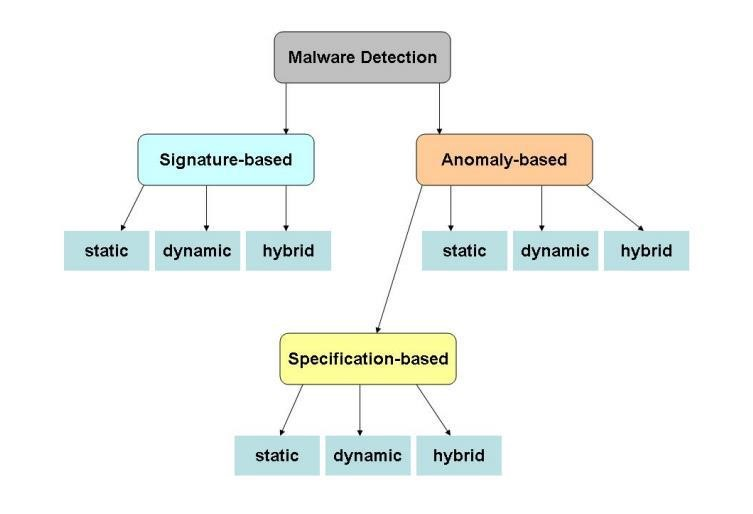
\includegraphics[scale=0.8]{figs/fig1}
\label{f.metodos_deteccao_01}
\legend{\small Fonte: Elaborada pelo autor.}
\end{figure}

\chapter{Problema}
\label{c.problema}

Os dispositivos móveis atuais ainda não possuem capacidade computacional de
sobra para que se façam varreduras constantes que utilizem as técnicas de
detecção dinâmicas em seus respectivos sistemas à procura de código malicioso,
e com a abrangência da internet se tornando cada vez mais expressiva, o dano
em potencial que um malware pode causar a um determinado indivíduo, ou ainda
em grupos massivos também torna-se mais preocupante. Sob a ótica de Szewczyk
(\citeyear{szewczyk12}), as redes de computadores, principalmente sem fio, começam a apresentar
problemas de vulnerabilidade a partir do momento da compra do \textit{hardware}
necessário para implementação da rede e da configuração desse equipamento,
onde muitas vezes os vendedores destes produtos tentam passar a ideia de que
os equipamentos por si são capazes de blindar uma rede contra qualquer
intrusão, a fim de obter sucesso comercial valendo-se da ingenuidade de
usuários leigos no assunto de segurança de redes. As técnicas de detecção por
assinatura, apesar de não serem as mais eficazes à disposição, são muito mais
simples de se implementar e resolverem o problema da infecção por malwares
conhecidos ou ainda malwares novos com características semelhantes às dos
conhecidos.




%DOCUMENTAÇÃO DO TEX PRA QUANDO DER AQUELE BRANCO FODA
%
%
%Para iniciar a produção em .tex é necessário instalar os pacotes básicos da linguagem e seus compiladores. O %MiKTeX é um pacote básico para o Windows (miktex.org/download) e o MacTeX um pacote básico para o Mac (tug.org/%mactex) que contém o mínimo necessário de TeX/LaTeX para rodar. Ele já vem com os compiladores nativos da %linguagem e uma IDE (TeXworks, para edição do texto) que possui o compilador integrado.

%

%Normalmente é utilizado o modo pdfLaTeX + MakeIndex + BibTeX para compilar um arquivo .tex. Existem outros %formatos de compiladores, mas essa opção é capaz de gerar um .pdf automático após a compilação e ainda por cima %adicionar as funcionalidades do BibTeX (recursos para criação e montagem automática de fontes bibliográficas).

%

%Além disso, também é necessária a instalação do pacote abnTeX2. Esse tutorial https://github.com/abntex/abntex2/%wiki/Instalacao provém o passo a passo de como instalar cada componente do TeX, em qualquer sistema operacional (%Linux, Mac OS e Windows). Caso esteja utilizando o MiKTeX, ele é capaz de efetuar o download do pacote %automaticamente, apenas instale-o, abra o projeto.tex e compile-o, ele irá requisitar a autorização para baixar %automaticamente os pacotes que faltam para efetuar a compilação.

%

%Com tudo em mãos e o compilador funcionando, é hora de abrir o modelo (projeto.tex) e começar a escrever o %texto. É possível perceber no código a estrutura do arquivo e os campos possíveis de edição. Ao escrever o %texto, ele é escrito normalmente, sendo que existem diversos comandos para estilizá-lo, criar tabelas, figuras, %dentre outros. A seguir abordaremos os principais comandos e funções que podem ser utilizadas em um projeto %básico de TCC. Para outras funções e pacotes, procure no Google, a comunidade é ativa e provavelmente já deve %ter feito o que é de sua necessidade.

%

%O arquivo projeto.tex contém os pacotes e comandos básicos que definem a estrutura desse texto já no formato %requisitado pela ABNT. Dentro dele é possível ver que estamos importando outros dois arquivos .tex (introducao e %conclusao), ou seja, esses arquivos estão sendo basicamente concatenados com o comando ``input''. A divisão não %é necessária, mas pode ser que auxilie na escrita do texto  ao deixar as coisas mais separadas e organizadas, %não sendo um único arquivo cheio de linhas e linhas de código.

%

%\section{Modificadores de Texto}
%\label{s.modificador}
%
%Os modificadores de texto mais simples utilizados são o negrito (``textbf'') \textbf{texto em negrito} e o %itálico (``emph'') \emph{texto em itálico}.
%\textbf
%
%\section{Seções}
%\label{s.citacoes}
%
%Seções podem ser criadas a partir do comando ``section'' e hierarquizadas abaixo do capítulo principal. É %possível referenciá-las, por exemplo, Seção~\ref{s.citacoes} corresponde a seção atual em que estamos. Já se %quisermos referenciar alguma outra coisa, é só utilizarmos o comando ``ref'' presente no código desse texto, por %exemplo, Capítulo~\ref{c.introducao}.
%
%\subsection{Subseções}
%\label{ss.subsecao}
%
%Subseções também podem ser criadas com o comando ``subsection'' e referenciadas~\ref{ss.subsecao}.
%
%\subsubsection{Sub-subseções}
%\label{sss.subsubsecao}
%
%Também há mais um nível que pode ser criado com o comando ``subsubsection''.
%
%\section{Alíneas}
%\label{s.alineas}
%
%\begin{alineas}
%
%\item As alineas devem ser criadas desse modo, com o comando begin\{alineas\}. Isso é necessário para que %estejam no formato definido pelo pacote abnTeX2 e, consequentemente, no formato definido pela ABNT.
%
%\item Cada item da alínea pode ser invocado com um comando item.
%
%\item O fim de cada alínea é determinado por end\{alineas\}.
%
%\end{alineas}
%
%\section{Tabelas}
%\label{s.tabelas}
%
%As tabelas também podem ser referenciadas como se fossem seções ou figuras, por exemplo, esta é a Tabela~\ref{t.t%ransacao_mercado}.
%
%\begin{table}[h]
%\centering
%\begin{tabular}{c|c}
%\hline
%\textbf{\small TID} & \textbf{\small Conjunto de Itens}\\\hline \hline
%{\small 1} & {\small \{Pão, Leite\}}\\\hline
%{\small 2} & {\small \{Pão, Fralda, Cerveja, Ovos\}}\\\hline
%{\small 3} & {\small \{Leite, Fralda, Cerveja, Coca-Cola\}}\\\hline
%{\small 4} & {\small \{Pão, Leite, Fralda, Cerveja\}}\\\hline
%{\small 5} & {\small \{Pão, Leite, Fralda, Coca-Cola\}}\\\hline
%\end{tabular}
%\caption{Exemplo de transações de mercado.}
%\label{t.transacao_mercado}
%\end{table}
%
%Quando uma tabela é criada com begin\{table\}, ela é automaticamente adicionada à Lista de Tabelas.
%
%\section{Algoritmos}
%\label{s.algoritmos}
%
%O pacote nicealgo incluído nos arquivos desse projeto é responsável por disponibilizar comandos extras, não %inerentes ao básico TeX, para a criação de algoritmos. Um exemplo do Algoritmo~\ref{a.algoritmo} é escrito a %seguir. Eles também pode ser referenciados como se fossem tabelas ou figuras.
%
%\begin{nicealgo}{a.algoritmo}
%\naTITLE{Algoritmo AIS}
%\naPREAMBLE
%\naINPUT{Conjunto Frequente L = 0 e Grupo de Fronteira F = 0.}
%\naBODY
%\naBEGIN{\textbf{Enquanto} $F \neq 0$, \textbf{faça}}
%\na{\textbf{Seja} conjunto candidato $C = 0$;}
%\naBEGIN{\textbf{Para cada} tuplas $t$ da base de dados, \textbf{faça}}
%\naBEGIN{\textbf{Para cada} conjuntos de itens $f$ em $F$, \textbf{faça}}
%\naBEGIN{\textbf{Se} $t$ contém $f$, \textbf{então}}
%\naEND{\textbf{Seja} $C_f =$ conjuntos de itens candidatos extensões de $f$ e contidos em $t$;}
%\naBEGIN{\textbf{Para cada} conjunto de itens $c_f$ em $C_f$, \textbf{faça}}
%\naBEGIN{\textbf{Se} $c_f \in C$, \textbf{então}}
%\naEND{$c_f$.contagem $= c_f$.contagem$ + 1$;}
%\naBEGIN{\textbf{Se não}}
%\na{$c_f$.contagem $= 0$;}
%\naEND{$C = C + c_f$;}
%\naEND{}
%\naEND{}
%\naEND{}
%\na{\textbf{Seja} F = 0;}
%\naBEGIN{\textbf{Para cada} conjunto de itens $c$ em $C$, \textbf{faça}}
%\naBEGIN{\textbf{Se} $contagem(c)/tamanho\_db > minsupport$, \textbf{então}}
%\naEND{$L = L + c$;}
%\naBEGIN{\textbf{Se} $c$ deve ser usado como a próxima fronteira, \textbf{então}}
%\naEND{$F = F + c$;}
%\naEND{}
%\naEND{}
%\end{nicealgo}
%
%\section{Figuras}
%\label{s.figuras}
%
%Abaixo podemos identificar a criação e referência da Figura~\ref{f.disposicao_mercado}. Atente-se ao código para
%perceber um possível redimensionamento com a função scale e o caminho de onde a figura deve ser retirada.
%
%Quando uma figura é criada com begin\{figure\}, ela é automaticamente adicionada à Lista de Ilustrações.
%
%\begin{figure}[h]
%\caption{\small Exemplo do ambiente TeXworks.}
%\centering
%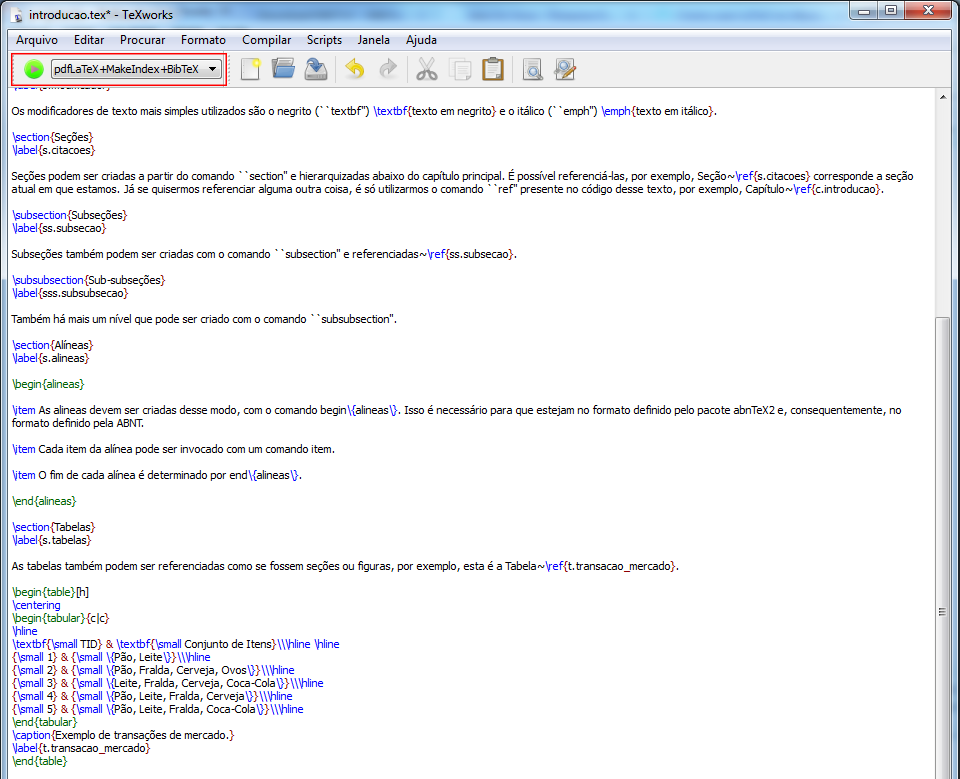
\includegraphics[scale=0.50]{figs/tex_exemplo.png}
%\label{f.disposicao_mercado}
%\legend{\small Fonte: Elaborada pelo autor.}
%\end{figure}
%
%\section{Equações}
%\label{s.equacoes}
%
%\section{Como citar as referências}
%\label{ss.referencias}
%
%Aqui está um exemplo de como podemos referenciar as bibliografias utilizadas no trabalho. Elas são guardadas na %forma de metadados (tags) no arquivo .bib a qual é importada no projeto principal (projeto.tex).
%
%E podemos citá-las de acordo com os identificadores atribuídos para cada referência, por exemplo,~\cite{%stonebraker93} e~\cite{rocha09}.
%
%Após citar um item de referência bibliográfica com o comando ``cite'', ela será automaticamente padronizada e %incluída na página de Referências de seu arquivo. Atualmente os maiores sites portadores de artigos, periódicos,
%dentre outros (IEEE, Springer, etc) já conseguem exportar a publicação desejado no formato BibTeX, sendo facilmente adicionado ao arquivo .bib de seu trabalho.
